% !TeX spellcheck = de_CH
%%%%%%%%%%%%%%%%%%%%%%%%%%%%%%%%%%%%%%%%%%%%%%%%%%%%%%%%%%%%%%%%%
%  _____   ____  _____                                          %
% |_   _| /  __||  __ \    Institute of Computitional Physics   %
%   | |  |  /   | |__) |   Zuercher Hochschule Winterthur       %
%   | |  | (    |  ___/    (University of Applied Sciences)     %
%  _| |_ |  \__ | |        8401 Winterthur, Switzerland         %
% |_____| \____||_|                                             %
%%%%%%%%%%%%%%%%%%%%%%%%%%%%%%%%%%%%%%%%%%%%%%%%%%%%%%%%%%%%%%%%%
%
% Project     : BA Welti Keller
% Title       : 
% File        : software.tex Rev. 00
% Date        : 15.09.2014
% Author      : Tobias Welti
%
%%%%%%%%%%%%%%%%%%%%%%%%%%%%%%%%%%%%%%%%%%%%%%%%%%%%%%%%%%%%%%%%%

\chapter{Software-Konzept}\label{chap.software}
\todo{software}

\section{Software-Stack}\label{sec.sw_stack}


\subsection{Überblick}\label{subsec.sw_ueberblick}
\todo{TK kurzbeschrieb über die softwarestruktur anhand der zwei Schemata}

\begin{figure}
	\centering
		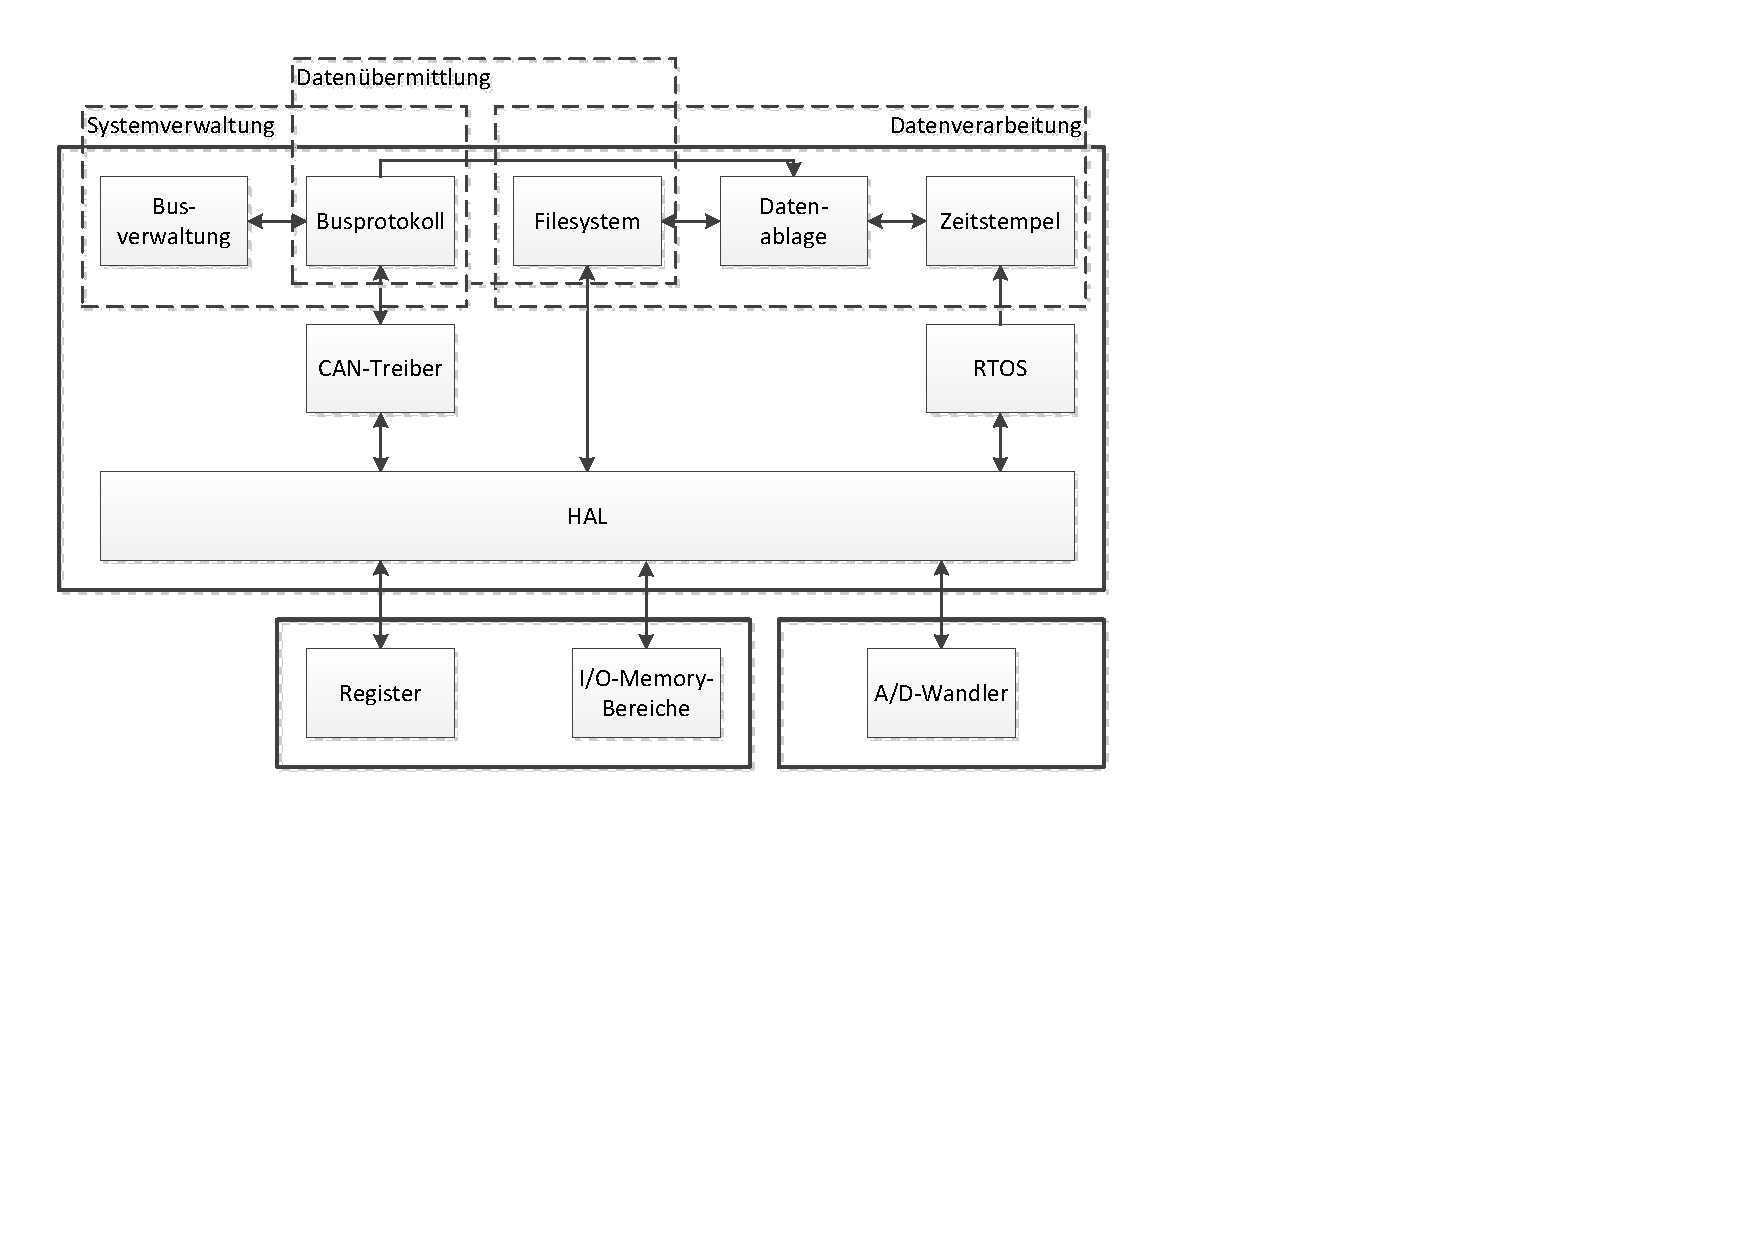
\includegraphics[width=0.8\textwidth]{images/visio/Softwarestack_Logger.pdf}
	\caption{Softwarestack des \gls{logger}s.}
	\label{fig.sw_logger}
\end{figure}

\begin{figure}
	\centering
		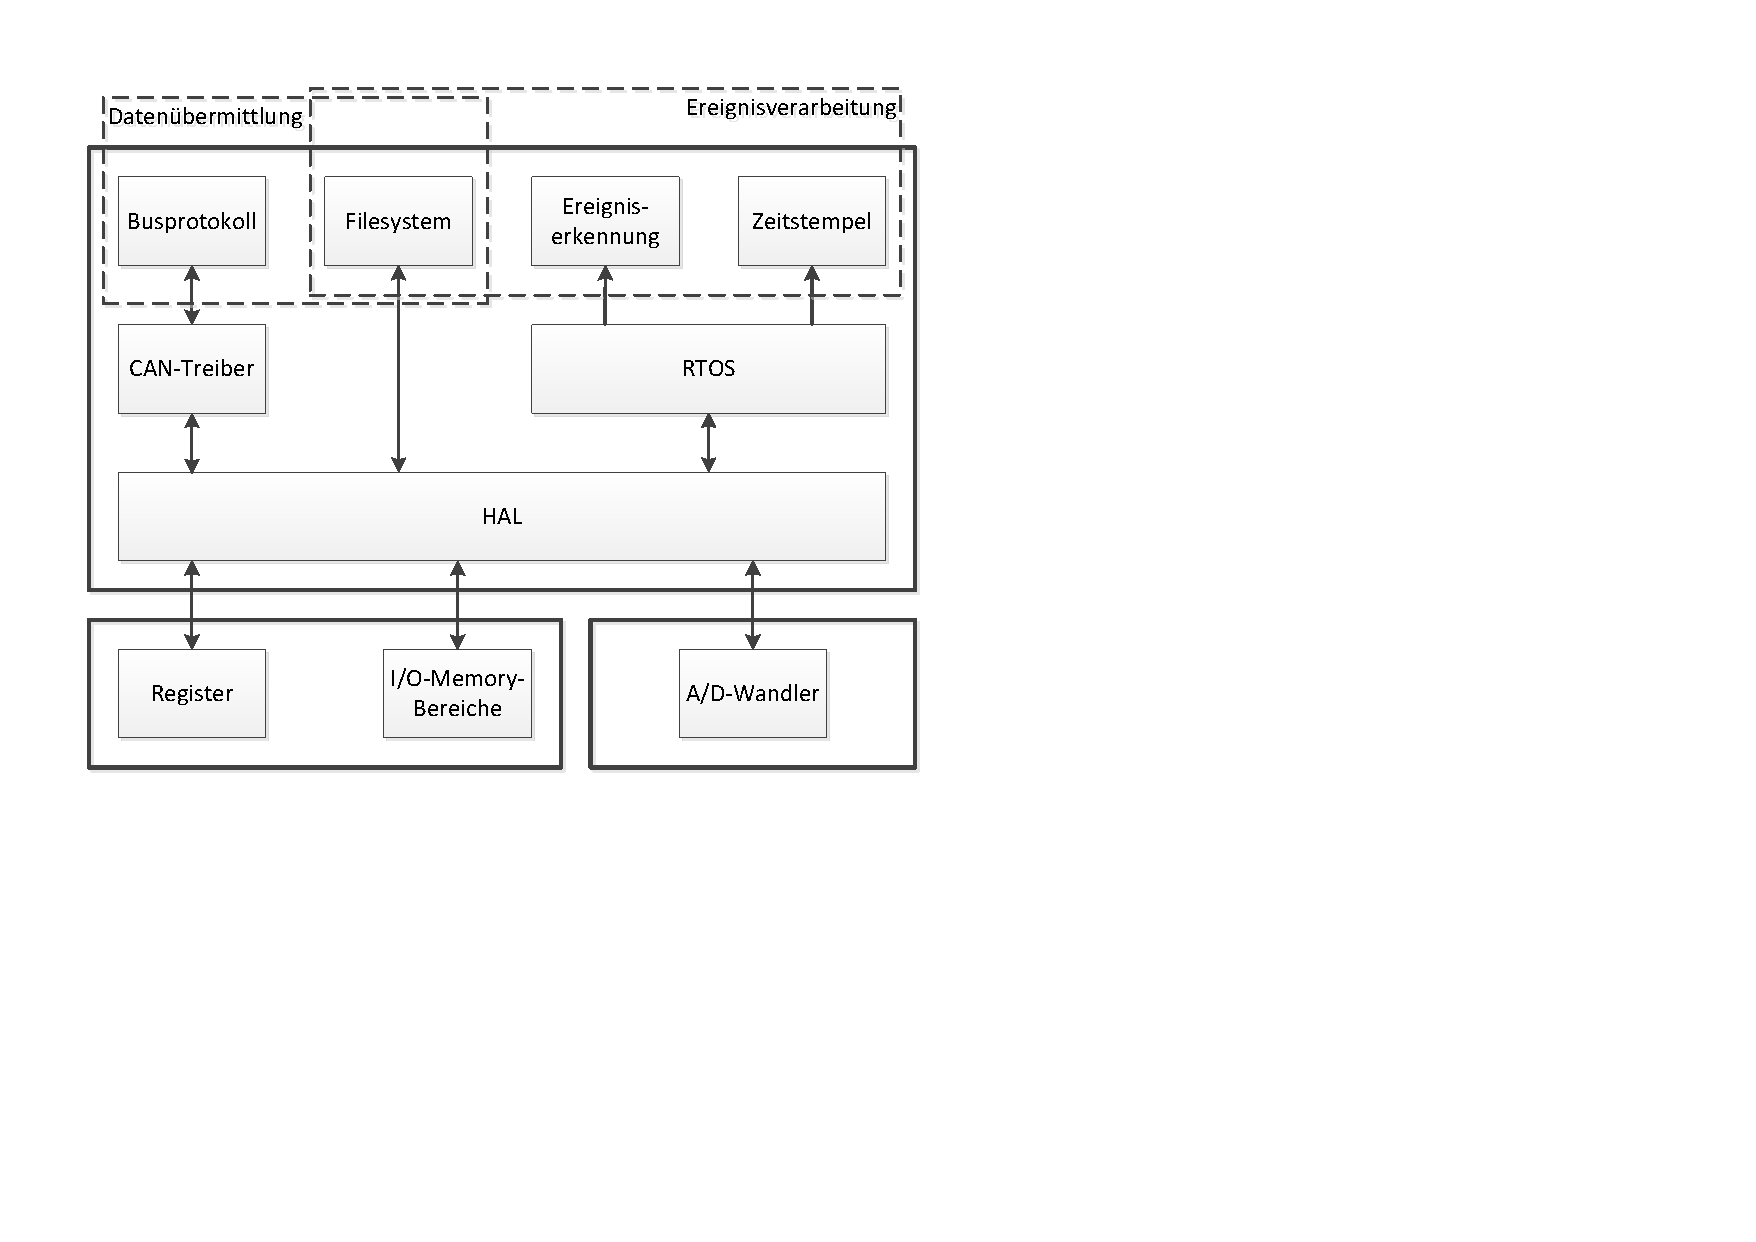
\includegraphics[width=0.8\textwidth]{images/visio/Softwarestack_Sensor.pdf}
	\caption{Softwarestack der \gls{sensoreinh}.}
	\label{fig.sw_sensor}
\end{figure}



\subsection{Messdatenerfassung}\label{subsec.sw_messen}
Der NXP LPC4088 Mikroprozessor verfügt über einen 12-bit \gls{adwandler}, der über einen Multiplexer auf acht \glspl{pin} messen kann. Auf dem verwendeten Quickstart-Board stehen sechs \glspl{pin} für A/D-Wandlung zur Verfügung. Für die geplante Anwendung reicht ein A/D-Pin, da der Beschleunigungs-\gls{sensor} die Beschleunigung nur auf einer Achse misst. Der \gls{adwandler} des NXP LPC4088 wird mit einer \gls{fs} von 10~kHz betrieben. Falls höhere \glspl{fs} nötig sind, kann der \gls{adwandler} theoretisch mit bis zu 400~kHz betrieben werden.

\paragraph{Abtastrate} Um die \gls{fs} genau einzuhalten wird ein Timer des \emph{NXP LPC4088} \gls{mc}s eingesetzt, der die Messung des \gls{adwandler}s anstösst (Listing \ref{list.tickerADC}). Die A/D-Wandlung nimmt immer genau 31 Taktzyklen in Anspruch. Nach abgeschlossener Messung schreibt der \gls{adwandler} den Messwert in ein eigenes Register und setzt einen \gls{irq}. Der \gls{irq} signalisiert dem \gls{mc}, dass ein Messwert zur Abholung bereit liegt. Damit der Messwert so rasch wie möglich, auf jeden Fall aber vor Ablauf der nächsten Messperiode, für die weitere Verarbeitung abgeholt werden kann, hat der \gls{irq} die höchst mögliche Priorität. Der Interrupt des \gls{adwandler}s unterbricht also jeden laufenden Prozess.

\begin{lstlisting}[caption=Timer mit Aufruf der A/D-Wandler-Funktion (ADC\_4088.cpp), label=list.tickerADC]
// ISR 
void start_ADC_Conversion(){
		// start conversion when the ticker fires
		LPC_ADC->CR |=(1 << 24);
}

// ...
// register Interrupt Handler and attach ticker
int register_ADC_interrupt(analogin_s *obj, PinName pin, uint32_t ADC_IRQHandler, uint32_t interval){
  // ...
  ticker.attach_us(&start_ADC_Conversion, interval);
  // ...
}
\end{lstlisting}

\paragraph{ISR} Der \gls{mc} ruft die \gls{isr} (Listing \ref{list.isrADC}) auf, um den \gls{irq} abzuhandeln. Die \gls{isr} holt den Messwert aus dem Register und speichert ihn zusammen mit dem \gls{timestamp} in einer \gls{fifo} ab. Die \gls{isr} erhöht den \gls{timestamp} um eins für den nächsten Messwert und gibt dann die Kontrolle an den unterbrochenen Prozess zurück.

\begin{lstlisting}[caption=ISR zur Abhandlung des ADC-Interrupt Requests (impact\_event.cpp), label=list.isrADC]
void isr_nextMeasurement(){
	// read ADC measurement from Register, automatically resets IRQ
	value = LPC_ADC->GDR;
	value = (value >> 4) & 0xFFF;
	timestamp++;
	
	enqueue_impact_input(timestamp, value);
}
\end{lstlisting}

\paragraph{Timestamp} Der Timestamp muss zwingend in der \gls{isr} (Listing \ref{list.isrADC}) erhöht werden, damit er immer sofort nach der Erfassung eines neuen Messwerts aktualisiert wird. Würde der Timestamp mittels einem zweiten Timer und einer zweiten \gls{isr} erhöht, bestünde die Gefahr einer ungeregelten Reihenfolge der Abarbeitung der \gls{irq}s. Mal würde der \gls{timestamp} vor dem Kopieren der Messdaten erhöht, mal erst danach.

\paragraph{Datenauswertung} Die Datenauswertung wird in regelmässigen Abständen aufgerufen und arbeitet die \gls{fifo} mit den neuen Messwerten ab, um Ereignisse zu erkennen. Der Aufruf der \gls{ereignisdet} ist nicht so stark an einen genauen Takt gebunden wie die A/D-Wandlung, da die \gls{fifo} genügend gross ist, um mehrere hundert Messwerte zwischenzuspeichern. Ein Thread ruft die \gls{ereignisdet} auf und wartet nach Beendigung der Subroutine 1~ms.

\subsection{Ereigniserkennung}\label{subsec.sw_ereignis}
\subsubsection{Hilbert-Transformation}
Von der \gls{wsl} wurde die \gls{ereignisdet} bisher mittels \gls{hilbert} gelöst. Die \gls{hilbert} liefert die umhüllende Kurve des gemessenen \gls{signal}s. Überschreitet die Umhüllende den \gls{threshold}, markiert dies den Start eines neuen \gls{ereignis}ses. Fällt die Umhüllende unter den \gls{threshold}, ist das \gls{ereignis} beendet. Abbildung \ref{fig.wslcurve} zeigt ein Beispiel von Messdaten aus einer bestehenden Anlage. Die Hüllkurve wurde von Hand eingezeichnet, um das Verfahren zu demonstrieren. Die \glspl{ereignis} werden als 'packet' bezeichnet, die Peaks als 'Impulses'.

\begin{figure}
	\centering
		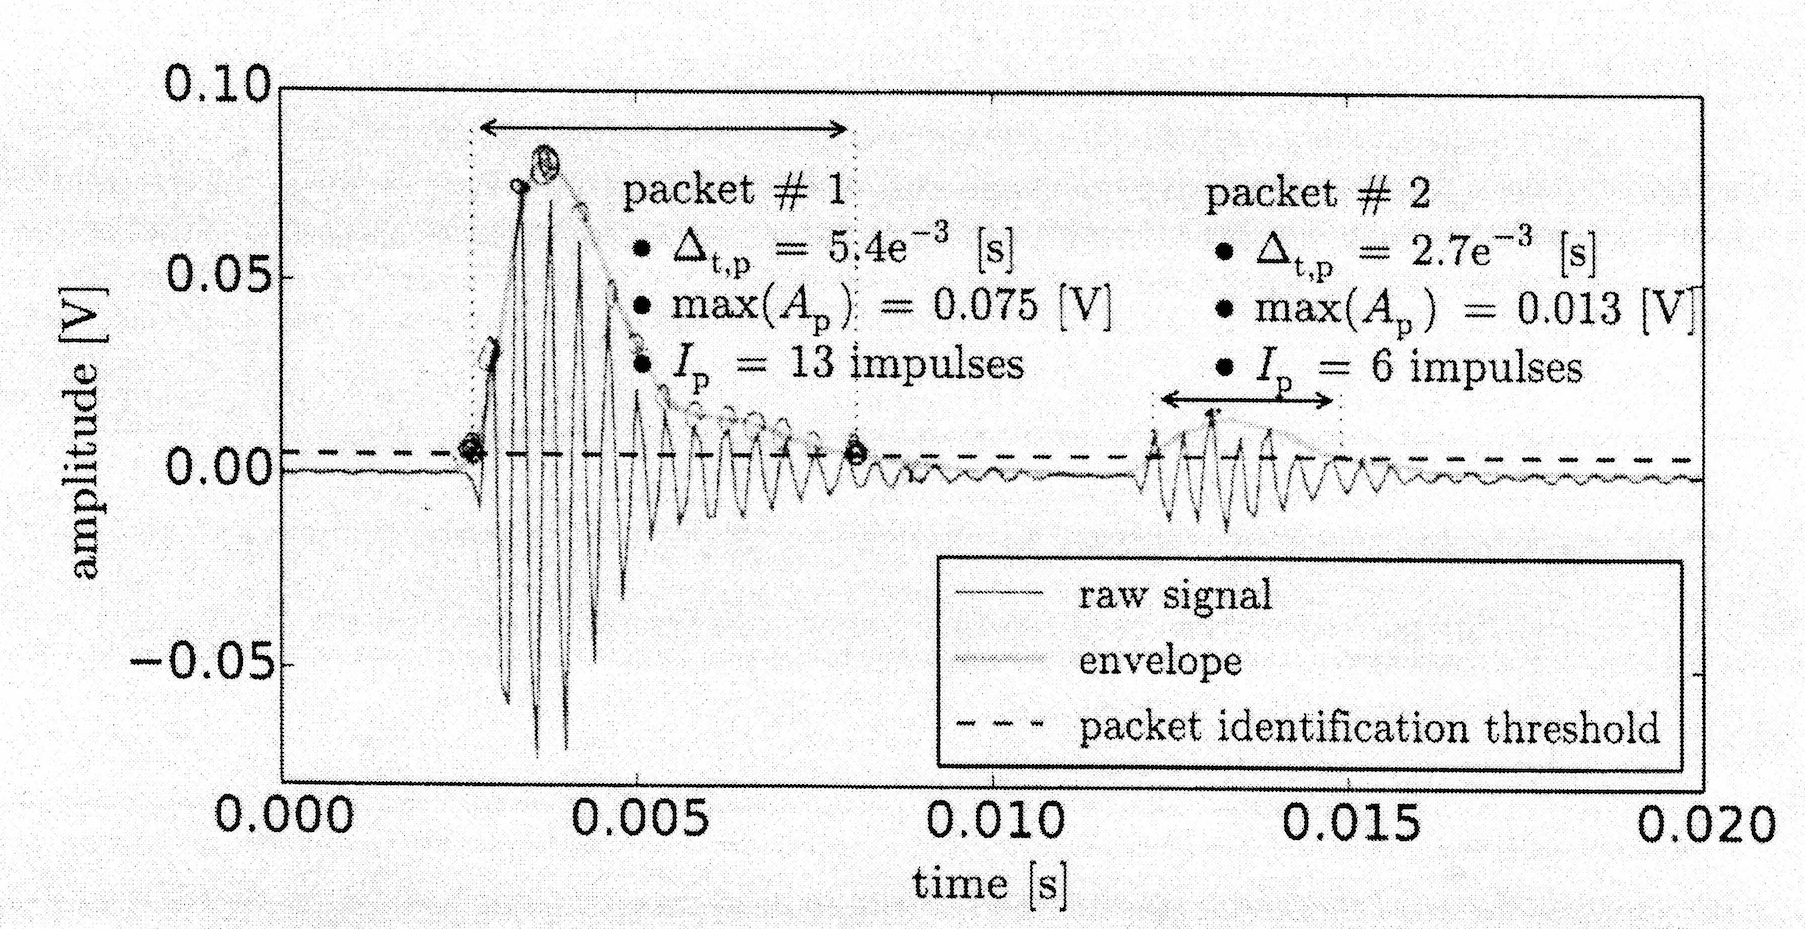
\includegraphics[width=0.8\textwidth]{images/curve_wsl.png}
	\caption{Beispiel von Messdaten mit einer Hüllkurve (envelope).}
	\label{fig.wslcurve}
\end{figure}

Die Berechnung der \gls{hilbert} erfordert einigen Aufwand. Mittels \gls{dft} wird das Spektrum des Signals berechnet. Negative Frequenzanteile werden auf null gesetzt und das resultierende Spektrum mittels \gls{idft} wieder in ein Signal umgerechnet (vgl. \cite{wiki_hilbert}). Das resultierende Signal umhüllt das Eingangssignal. 

Für die \gls{dft} und die \gls{idft} ist der Rechenaufwand je \ensuremath{N \cdot log_2(N)}. Je mehr Datenpunkte in einem Schritt verrechnet werden (\gls{blockg}), desto höher ist der Aufwand, aber desto genauer ist das Resultat. Mit einer \gls{blockg} von 128 Messwerten benötigt die \gls{dft} und die \gls{idft} je 896 komplexe Multiplikationen und Additionen (vgl. \cite[Kap. 3, S. 48]{dsv1_hilbert}). Pro Messwert sind das 7 komplexe Multiplikationen und Additionen. Dank der DSP-Fähigkeiten des gewählten Cortex\texttrademark -M4 Prozessors liegt die zu erwartende Prozessorauslastung für die \gls{hilbert} bei einer \gls{fs} von \ensuremath{10~kHz} bei wenigen Prozent.

\subsubsection{Hilbert-Transformation als FIR-Filter}
Die \gls{hilbert} kann mittels eines \gls{fir}s angenähert werden. Ein Allpass mit gerader Filter-Ordnung und geeignet gewählten Koeffizienten (Abbildung \ref{fig.hilbertFIR}) liefert eine gute Näherung. Je nach gewählter Ordnung des Filters ist der Rechenaufwand aber in ähnlicher Grössenordnung wie mit \gls{dft} und \gls{idft}.
\begin{figure}
	\centering
		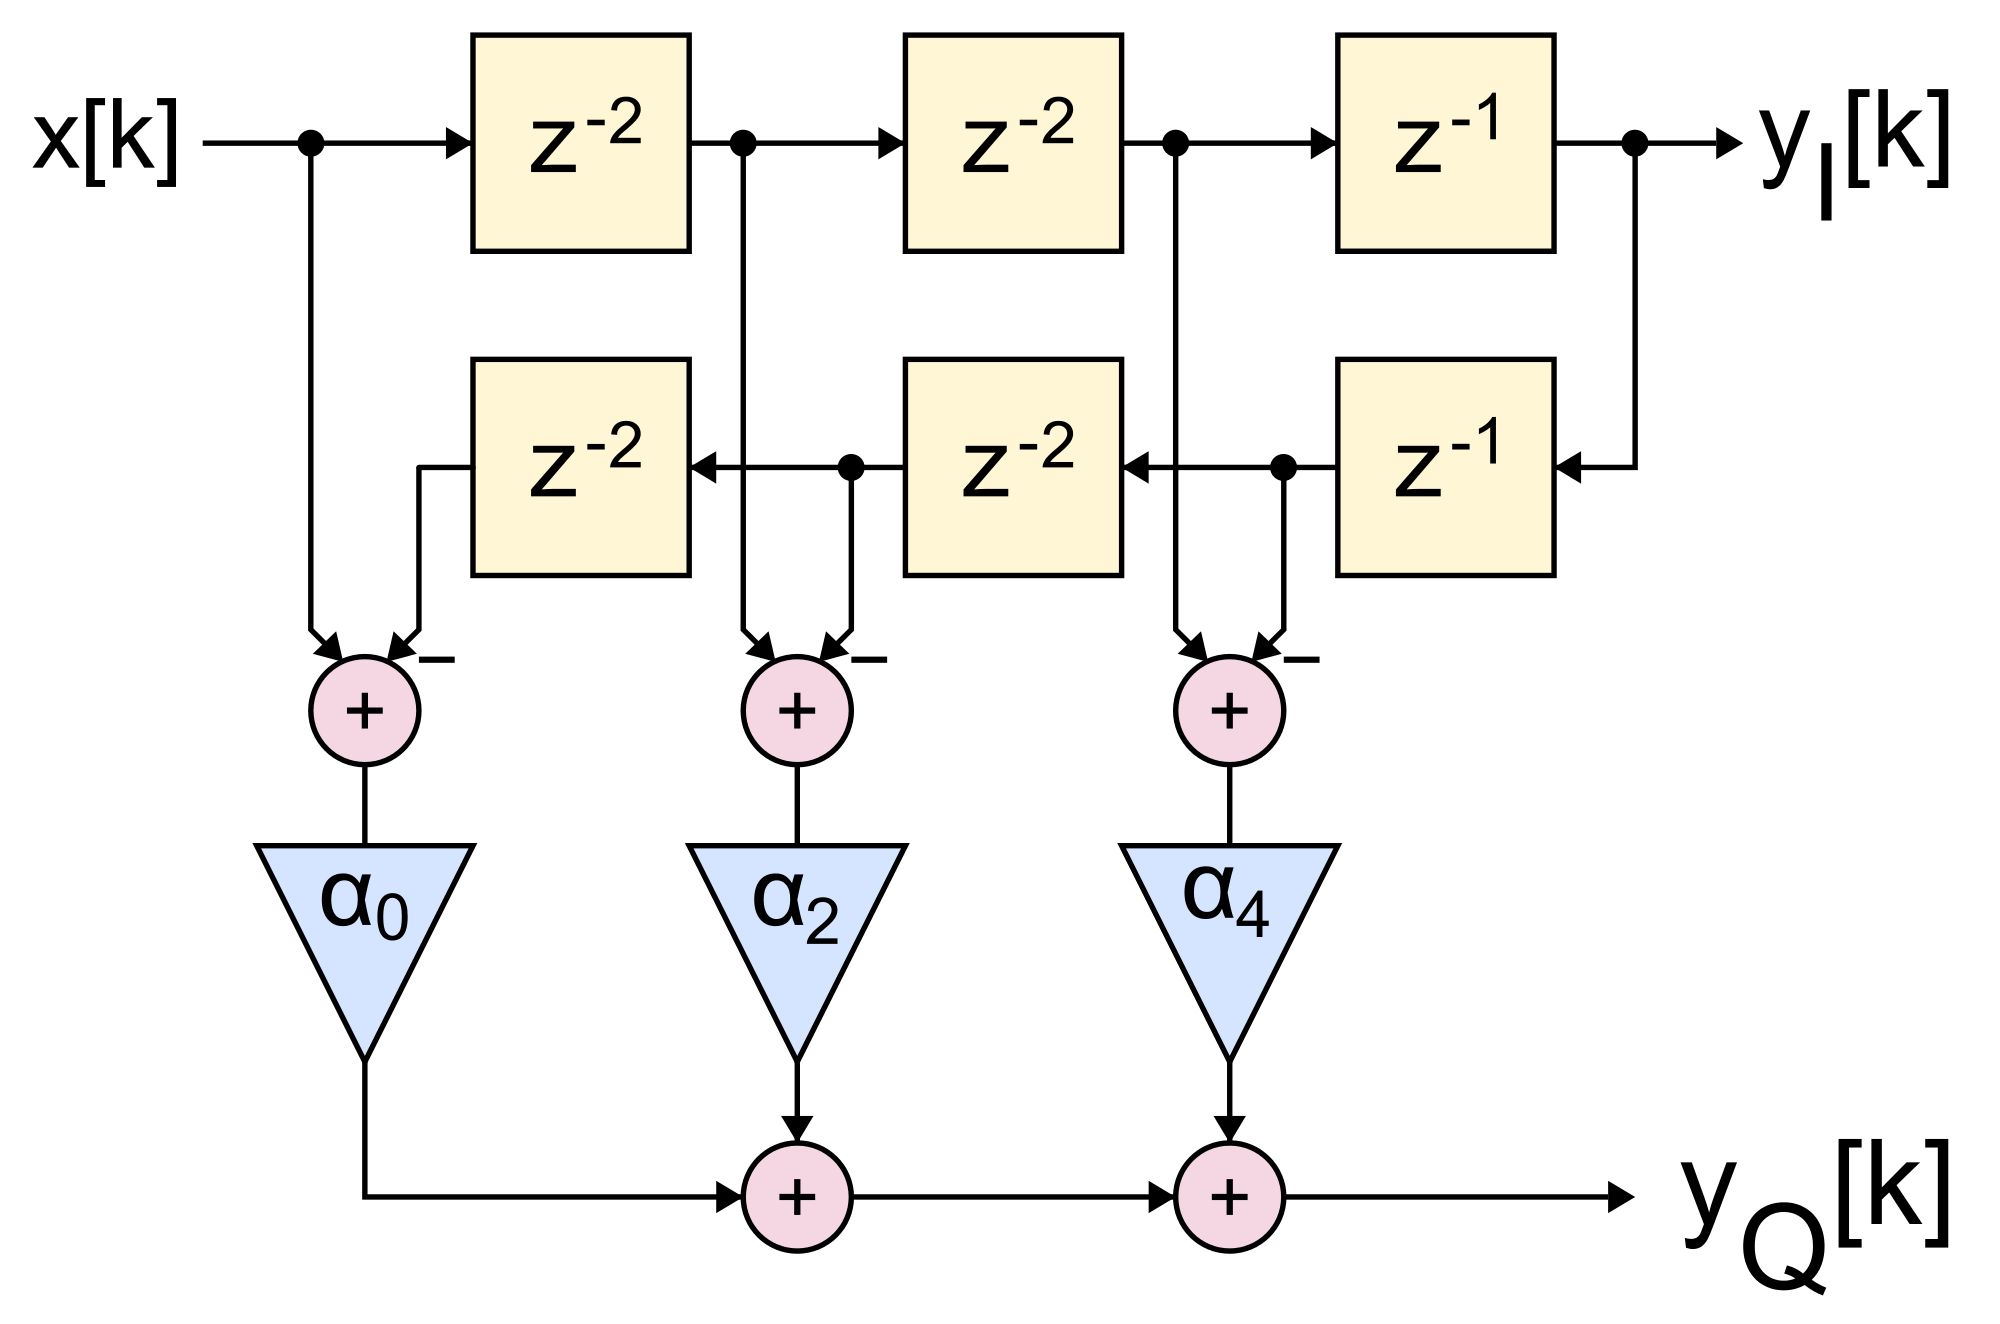
\includegraphics[width=0.8\textwidth]{images/FIR_Hilbert_Transform_Filter.png}
	\caption{\gls{hilbert} als \gls{fir} \cite{wiki_hilbertFIR}.}
	\label{fig.hilbertFIR}
\end{figure}

\subsubsection{Zustandsmaschine}
Um den Rechenaufwand der Hilbert-Transformation zu umgehen, lösen wir die \gls{ereignisdet} mittels einer \gls{fsm}. Das Zustandsdiagramm der \gls{fsmgloss} in Abbildung \ref{fig.fsm_impact_detection} zeigt alle möglichen Zustände der \gls{fsm} und welche Ereignisse einen Übergang in einen anderen Zustand auslösen.

\begin{figure}
	\centering
		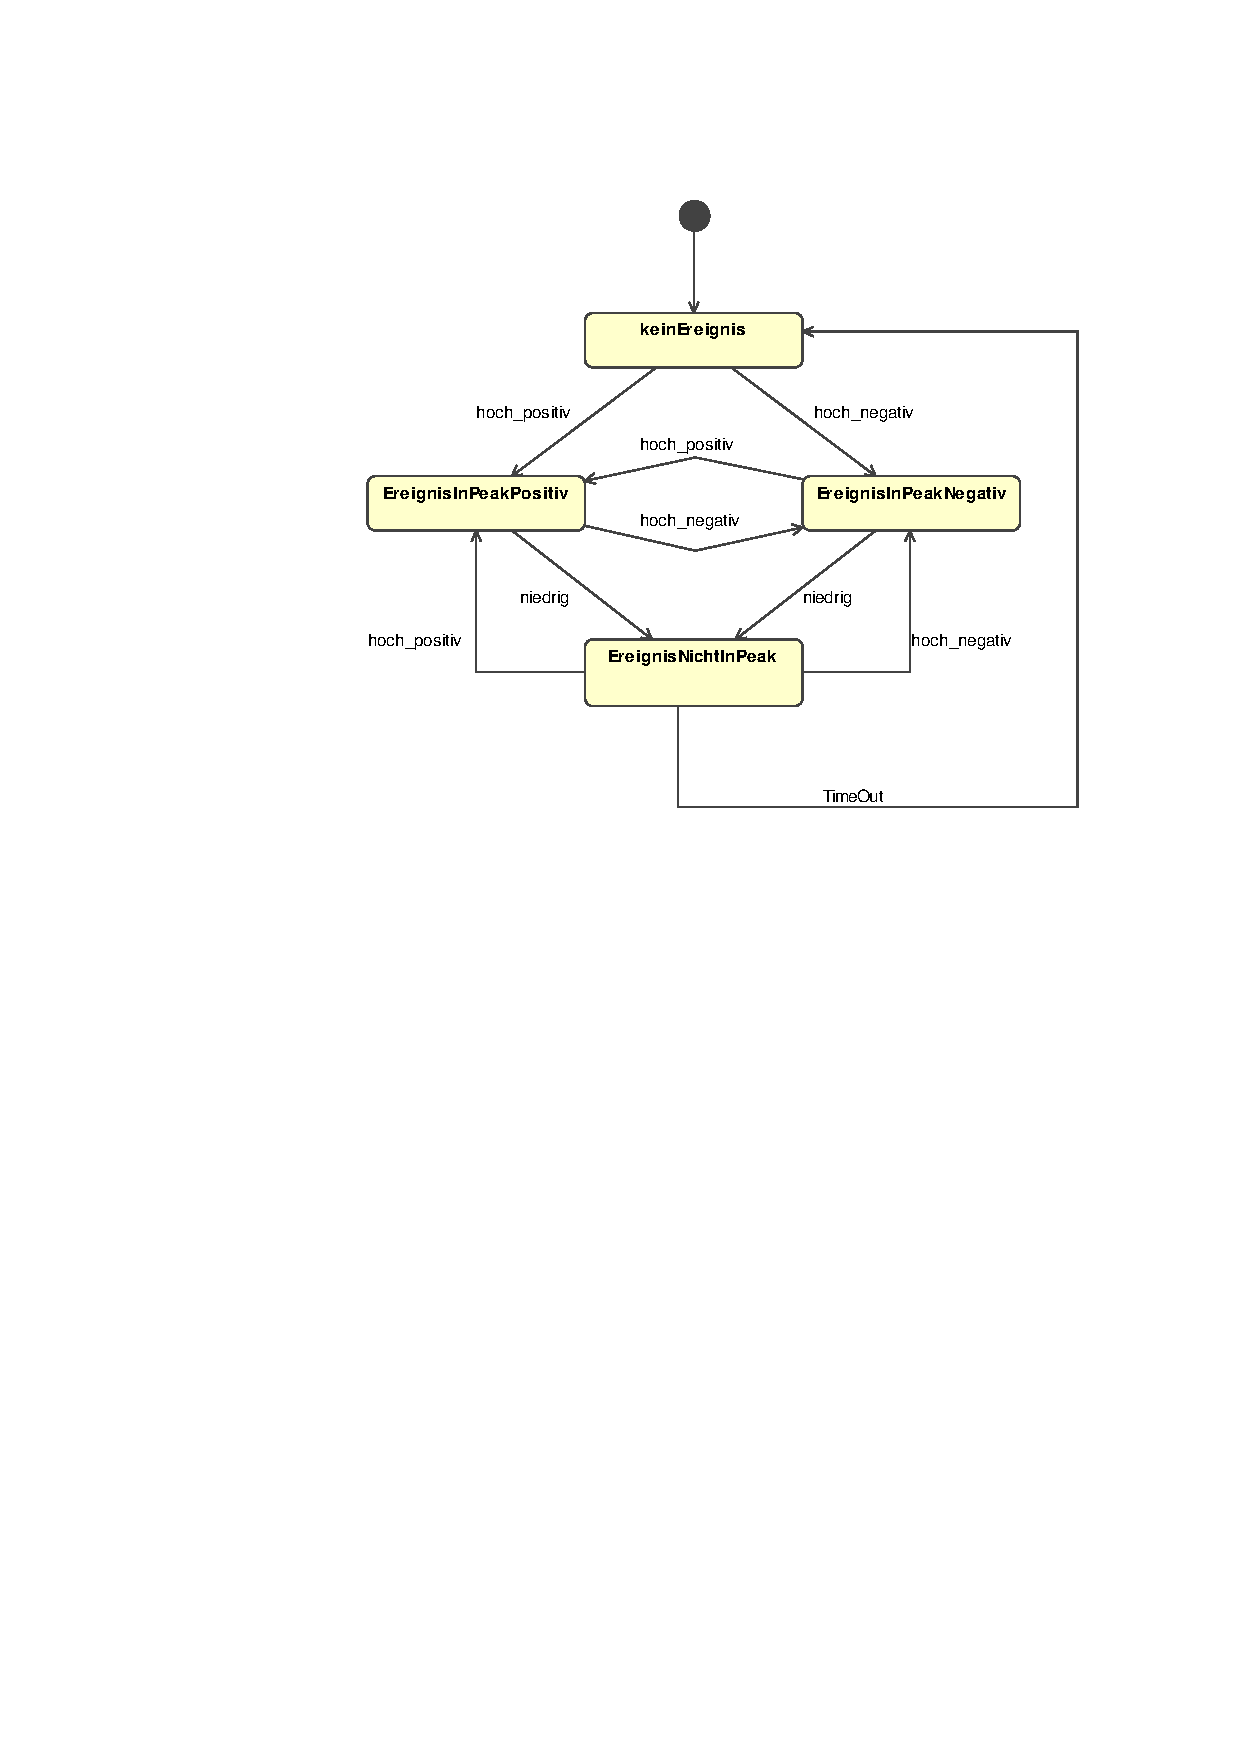
\includegraphics[width=0.8\textwidth]{images/magicdraw/Ereigniserkennung.pdf}
	\caption{Zustandsmaschine der Ereigniserkennung.}
	\label{fig.fsm_impact_detection}
\end{figure}

\paragraph{Konfiguration der Zustandsmaschine}
 Über Parameter wird definiert, welche Signalform als \gls{ereignis} erkannt werden soll. In Abbildung \ref{fig.impact_detection_params} sind die Parameter dargestellt. 
\begin{figure}
	\centering
	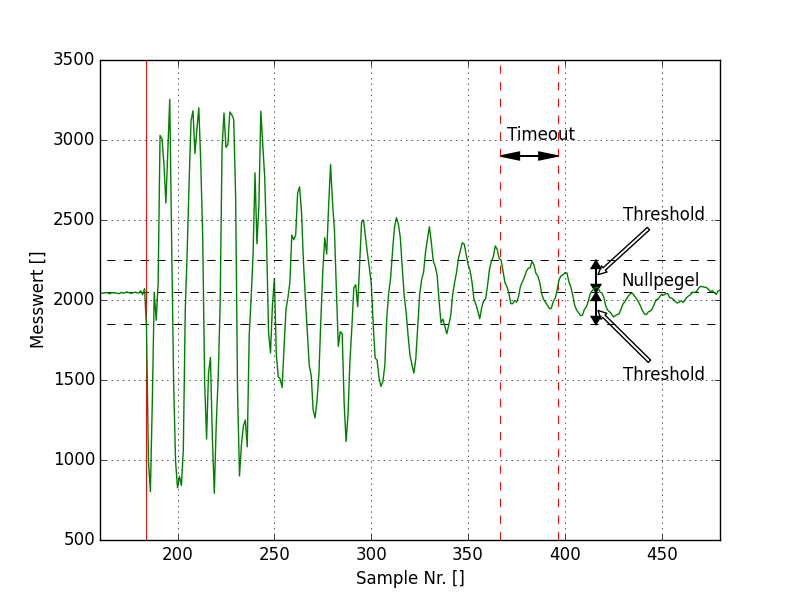
\includegraphics[width=0.8\textwidth]{images/impact_params.png}
	\caption{Parameter der Ereigniserkennung.}
	\label{fig.impact_detection_params}
\end{figure}

\paragraph{Nullpegel} Der \gls{nullpegel} kann angepasst werden, um die Erdanziehung, die als Beschleunigung auf den Sensor wirkt, zu kompensieren. Je nachdem wie der Sensor orientiert ist, ist die Erdanziehungskraft nicht parallel zur Mess-Achse des Sensors. Die vom Sensor gemessene Erdanziehungskraft in Richtung der Mess-Achse ist damit nicht immer gleich gross. Deshalb muss der \gls{nullpegel} angepasst werden können. Die mittlere gestrichelte schwarze Linie in Abbildung \ref{fig.impact_detection_params} stellt den \gls{nullpegel} dar.

\paragraph{Threshold} Der \gls{threshold} definiert, ab welcher Abweichung des Signalpegels vom Nullpegel die \gls{fsm} einen Messwert als 'hoch' betrachten soll. Zu beachten ist, dass der \gls{threshold} auf beide Seiten des Nullpegels gilt. Da der Sensor sowohl Beschleunigungen nach oben wie auch nach unten erfährt, unterscheidet die \gls{fsm} dies mit den Ereignissen 'hoch\_positiv' resp. 'hoch\_negativ'. Signalpegel, die den Threshold nicht überschreiten, werden als 'niedrig' eingestuft. In Abbildung \ref{fig.impact_detection_params} ist das erste Erreichen des (negativen) \gls{threshold}s mit einer vertikalen roten Linie markiert.

\paragraph{Timeout} Da ein Ereignis aus mehr als einem \gls{peak} besteht, muss eine Dauer (\gls{timeout}) definiert werden können, während der die \gls{fsm} auf den Beginn eines neuen \gls{peak}s wartet. Tritt während des \gls{timeout}s kein neuer Peak auf, gilt das Ereignis als beendet. Die gestrichelten roten Linien in Abbildung \ref{fig.impact_detection_params} zeigen den Timeout.

\subsubsection{Ablauf der Zustandsmaschine}
Im Folgenden wird der Ablauf in der Zustandsmaschine genauer erklärt. Im Zustandsdiagramm in Abbildung \ref{fig.fsm_impact_detection} sind die Namen der Zustände und Ereignisse ersichtlich. Der Übersichtlichkeit halber wurde auf die Auflistung der Aktionen im Diagramm verzichtet.

Die \gls{fsm} wird im Zustand 'keinEreignis' initialisiert. Tritt ein Messwert auf, der als 'hoch\_positiv' klassiert wird, wechselt die \gls{fsm} in den Zustand 'EreignisInPeakPositiv'. In diesem Zustand verbleibt die \gls{fsm}, bis ein anders klassierter Messwert eintrifft. 

Ein Messwert 'niedrig', also unterhalb des \gls{threshold}s, führt zu einem Übergang in den Zustand 'EreignisNichtInPeak'. Dieser Übergang startet einen Timer, der während der im Parameter 'Timeout' definierten Anzahl Messwerte läuft. Falls die \gls{fsm} bis zum Ablauf des Timers keinen Messwert 'hoch\_positiv' oder 'hoch\_negativ' erhält, wechselt sie wieder in den Zustand 'keinEreignis' und übergibt die Ereignisdaten dem Prozess, der für die Übertragung zum \gls{logger} zuständig ist. 

Der Timer läuft nicht in Echtzeit, sondern zählt die Anzahl Messwerte seit seinem Start, da die Verarbeitung asynchron zur Erfassung der Messwerte läuft. Das bedeutet, dass die Verarbeitung problemlos während mehreren Messwerten stillstehen kann, ohne dass Messwerte verloren gehen. Dies ist möglich, da die Messwerte in eine Warteschlange (\gls{fifo}) geschrieben werden, von wo sie von der \gls{fsm} abgeholt werden. So lange die \gls{fifo} nicht überfüllt wird, gehen keine Messwerte verloren. Die Verarbeitung der Messwerte in der \gls{fsm} erfolgt im \emph{NXP LPC4088} \gls{mc} schnell genug, um theoretisch mit einer \gls{fs} bis \ensuremath{200~kHz} messen zu können.

Falls die \gls{fifo} doch einmal überlaufen sollte, wird eine Nachricht an den \gls{logger} übertragen, der eine entsprechende Meldung in die Datendatei der \gls{sensoreinh} einträgt. Dies bedeutet, dass zu diesem Zeitpunkt einige Messwerte verloren gegangen sind. Da der \gls{timestamp} in der \gls{sensoreinh} trotzdem mit jedem \gls{sample} erhöht wird, stimmen die Zeitangaben in der Datendatei weiterhin. Es besteht lediglich eine Lücke im Datensatz.

\todo{TK: Zusammenhänge A/D-Wandlung und Ereigniserkennung und Übertragung beschreiben, dazu ein Kommunikationsdiagramm, wo synchron, wo asynchron.}

\subsection{Detail-Level}
Je nach Einsatz der Messstation variiert die benötigte unbeaufsichtigte Messdauer von einigen Tagen bis zu mehreren Monaten. Die zu speichernde Datenmenge muss an diese Dauer angepasst werden können. Für einen langen Einsatz werden von Vorteil weniger detaillierte Messdaten abgespeichert, während für einen eher kurzen Einsatz unter Umständen sogar unkomprimierte Daten abgespeichert werden können.

Für die Wahl einer geeigneten Datenrate stehen vier verschiedene Modi, sog. Detail-Level zur Verfügung. 

Im 'raw'-Modus werden Rohdaten gespeichert (Abbildung \ref{fig.det_raw}). Dieser Modus soll hauptsächlich der Gewinnung von Kalibrierungsdaten dienen, da hier sehr viele Daten anfallen. Es wird empfohlen, nur wenige Sensoren in diesen Modus zu versetzen.

Im 'detailed'-Modus werden von jedem Ereignis alle Datenpunkte gespeichert (Abbildung \ref{fig.det_det}. Die uninteressanten Datenpunkte zwischen den Ereignissen werden nicht übertragen und aufgezeichnet. Dieser Modus ist sowohl für kurze als auch für längere Messperioden interessant, da er nur interessante Daten aufzeichnet. Die Menge anfallender Daten hängt direkt von der Häufigkeit der Ereignisse ab.

Der 'peaks only'-Modus zeichnet die Dauer des \gls{ereignis}ses sowie Zeitpunkt und Intensität aller \gls{peak}s eines \gls{ereignis}ses auf. Damit ist ein grosser Teil der Information des 'detailed'-Modus vorhanden, aber in geringerer zeitlicher Auflösung.

Der 'sparse'-Modus liefert lediglich die Dauer des \gls{ereignis}ses, die Anzahl Peaks und den maximalen Ausschlag. Dies ist eine minimale Informationsmenge, die dennoch eine Aussage über das \gls{geschiebekorn} zulässt.

Eine ausführliche Beschreibung der Detail-Level ist in der Bedienungsanleitung ab Abschnitt \ref{ssec.detaillevel}, Seite \pageref{ssec.detaillevel} zu finden.

\begin{figure}
\centering
\begin{minipage}{0.5\textwidth}
\centering
		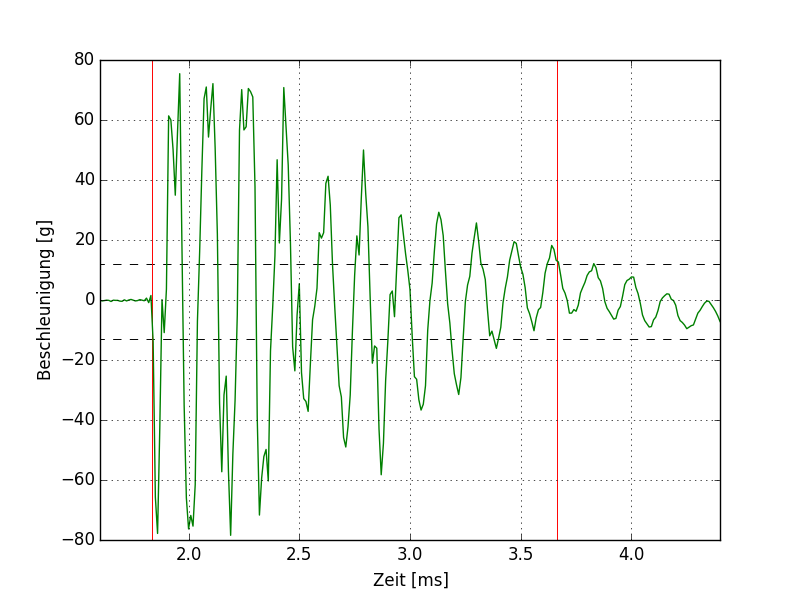
\includegraphics[width=0.95\textwidth]{images/rawshort.png}
	\captionof{figure}{Detail-Level 'raw'.}
	\label{fig.det_raw}
\end{minipage}%
\begin{minipage}{0.5\textwidth}
\centering
		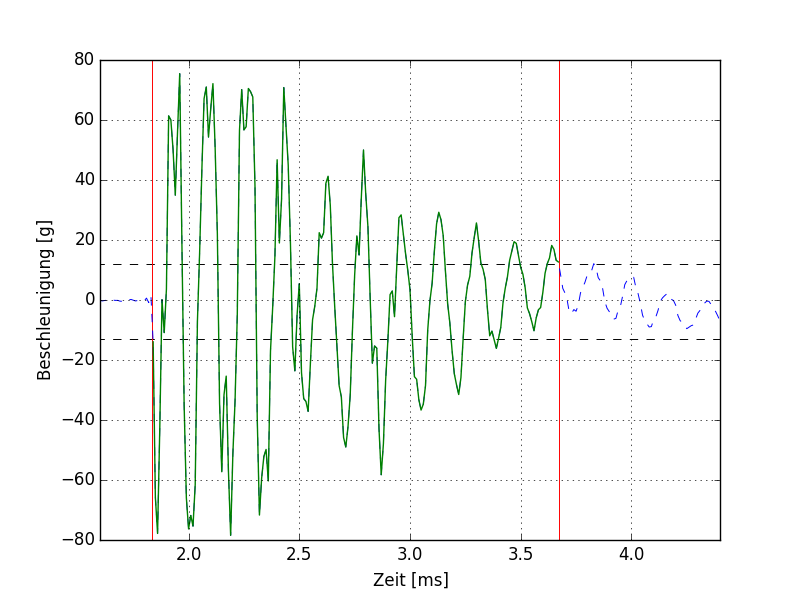
\includegraphics[width=0.95\textwidth]{images/detailed.png}
	\captionof{figure}{Detail-Level 'detailed'.}
	\label{fig.det_det}
\end{minipage}
\end{figure}

\begin{figure}
\centering
\begin{minipage}{0.5\textwidth}
\centering
		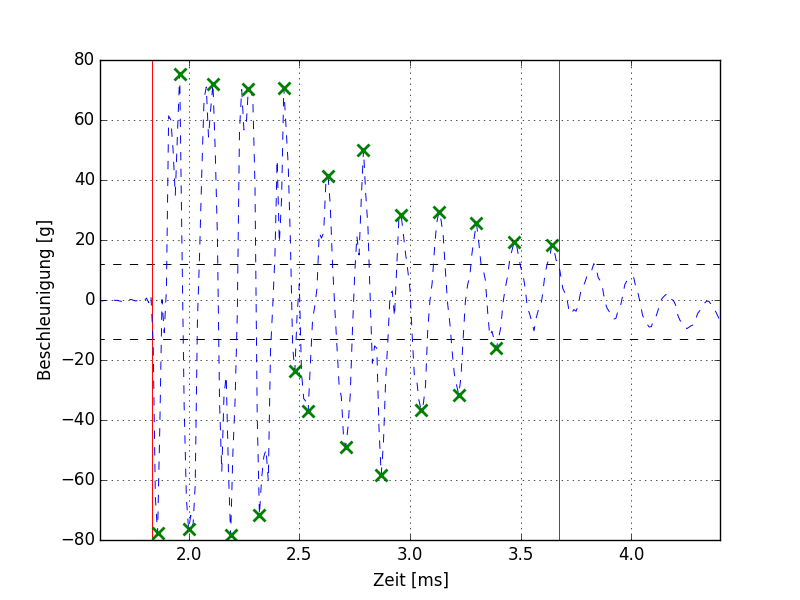
\includegraphics[width=0.95\textwidth]{images/peaks.png}
	\captionof{figure}{Detail-Level 'peaks only'.}
	\label{fig.det_peak}
\end{minipage}%
\begin{minipage}{0.5\textwidth}
\centering
		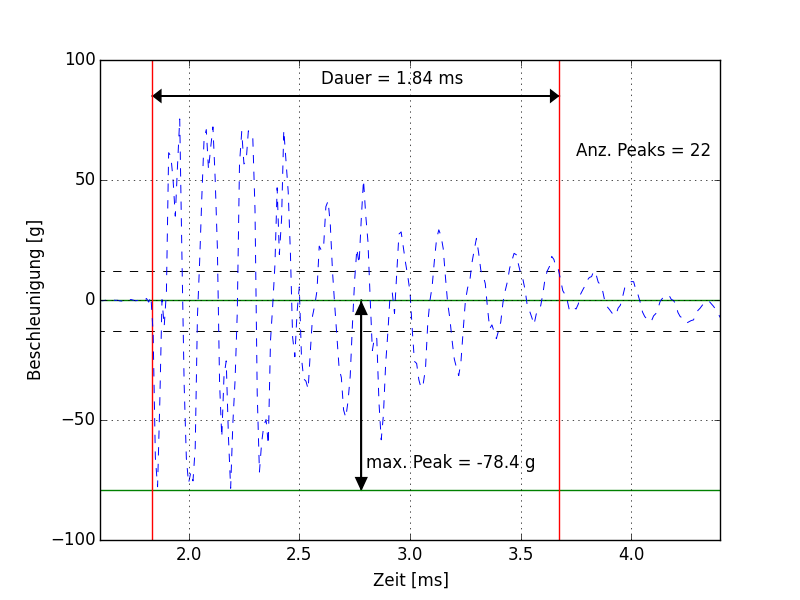
\includegraphics[width=0.95\textwidth]{images/sparse.png}
	\captionof{figure}{Detail-Level 'sparse'.}
	\label{fig.det_sparse}
\end{minipage}
\end{figure}



\subsection{Timestamp}\label{subsec.sw_timestamp}
Der \gls{timestamp} ist ein Zähler, der in jeder \gls{sensoreinh} die gemessenen \glspl{sample} zählt. Die übertragenen \glspl{ereignis} werden mit dem \gls{timestamp} versehen. Der \gls{logger} kann anhand des \gls{timestamp}s, der \gls{fs} der betreffenden \gls{sensoreinh} und des Zeitpunkts des letzten Zurücksetzens der \gls{timestamp}s den Zeitpunkt der Aufnahme des \gls{ereignis}ses berechnen (Gleichung \ref{eq.timestamp}).

\begin{equation}\label{eq.timestamp}
t_{Ereignis} = t_{reset} + (timestamp/fs)
\end{equation}

\section{Busverwaltung}

\subsection{Verwaltung des Bussystems}\label{subsec.sw_busverwaltung}

\todo{TK: Busverwaltung beschreiben}

\begin{figure}
	\centering
		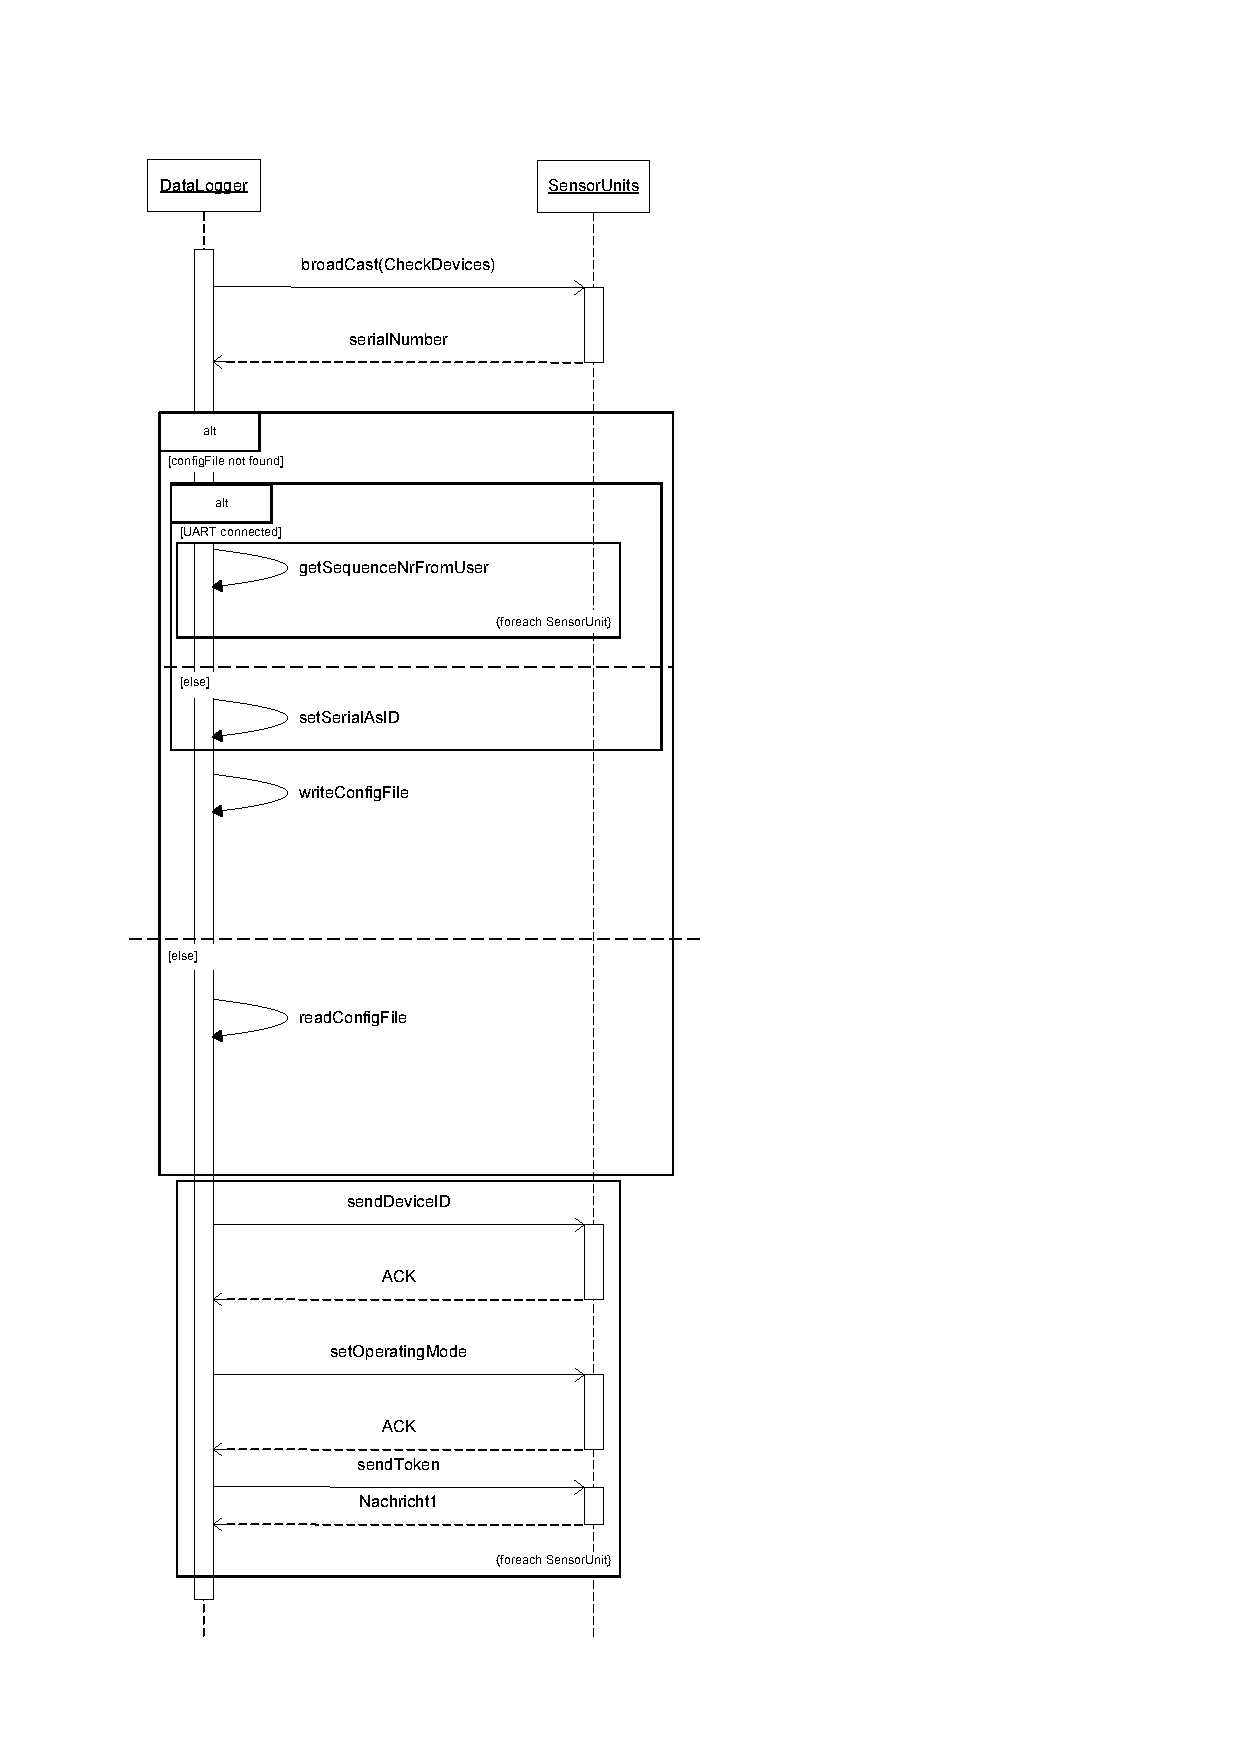
\includegraphics[height=0.9\textheight]{images/magicdraw/StartUpSequenz.pdf}
	\caption{Sequenzdiagramm des Startupvorgangs der Messstation.}
	\label{fig.seq_startup}
\end{figure}

\todo{TK: Figur \ref{fig.seq_startup} neu machen}

\subsection{Busprotokoll}\label{subsec.sw_busprotokoll}
\todo{TK: Busprotokoll}
\todo{TK: Kommunikationsdiagramm Bushandler}
\todo{TK: Interrupt-System des Bushandlers aufführen}

\subsection{Filesystem}\label{subsec.sw_filesystem}
Der \gls{logger} legt die Messdaten für jede \gls{sensoreinh} in eine eigene Datei ab. Die Filepointer werden zusammen mit den Konfigurationsdaten im Arbeitsspeicher gehalten. Beim Stoppen einer \gls{sensoreinh} wird die Datei geschlossen und beim erneuten Start der \gls{sensoreinh} eine neue Datei eröffnet. Beim Stopp/Start des \gls{logger}s erfolgt dies für alle Dateien.

Vor dem Entfernen der SD-Karte muss deshalb der \gls{logger} gestoppt werden. Zu diesem Zweck gibt es im Konfigurationsmenü einen eigenen Befehl 'unmount SD card'.

Die Dateinamen haben die Form 'sxx\_MMDD\_hhmm.dat', wobei 'xx' der CAN-ID entspricht, 'MMDD' dem Monat/Tag und 'hhmm' der Stunde/Minute des Starts.

Bei Konfigurationsänderungen schreibt der \gls{logger} einen entsprechenden Eintrag in die Sensordatei. Der Eintrag wird auf eine neue Zeile geschrieben und mit dem Symbol '\#' als Log-Eintrag markiert. Der Eintrag enthält die Uhrzeit und den neuen Wert des Parameters. Am '\#'-Symbol erkennt ein Auswertungsprogramm eine solche Informationszeile und kann diese ignorieren oder bei Bedarf auch entsprechend verarbeiten.



\section{Konfiguration}\label{sec.sw_konfiguration}
Die Konfiguration der Messstation erfolgt einerseits über die Datei 'config.txt', die sich auf der SD-Karte befindet. Andererseits steht über einen \gls{usb}-Anschluss eine serielle Schnittstelle zur Verfügung. Mit einem \gls{terminalemu} kann auf ein Konfigurationsmenü zugegriffen werden, um die Funktionen der Messstation zu steuern.

Die Verwendung der seriellen Schnittstelle über \gls{usb} ist in Abschnitt \ref{ssec.manualserial} der Bedienungsanleitung (ab Seite \pageref{ssec.manualserial}) beschrieben.

Die komplette Beschreibung des Konfigurationsmenüs befindet sich in der Bedienungsanleitung ab Abschnitt \ref{ssec.menu}, Seite \pageref{ssec.menu}.
